% N2 / design structure matrix for the two sizing loops, side by side.
%
% Reading rule: the cell in row i, column j is marked when component i sends
% something to component j. Marks ABOVE the diagonal are feed-forward. Marks
% BELOW the diagonal are FEEDBACK, and every one of them is a reason the
% process has to iterate.
\documentclass[border=8pt, tikz]{standalone}
\usepackage[T1]{fontenc}
\usepackage{lmodern}
\usepackage{amsmath}
\usetikzlibrary{matrix, positioning, fit, backgrounds}

\definecolor{n2Comp}{RGB}{200, 221, 242}
\definecolor{n2Fwd}{RGB}{212, 239, 213}
\definecolor{n2Back}{RGB}{240, 168, 148}

\tikzset{
  Cell/.style   = {draw=black!25, minimum size=9.5mm, anchor=center, font=\scriptsize},
  Comp/.style   = {Cell, fill=n2Comp, font=\scriptsize\bfseries},
  Fwd/.style    = {Cell, fill=n2Fwd},
  Back/.style   = {Cell, fill=n2Back, font=\scriptsize\bfseries},
  Empty/.style  = {Cell, fill=white},
  RowLab/.style = {font=\scriptsize, anchor=east, inner sep=2.5pt},
  ColLab/.style = {font=\scriptsize, anchor=west, rotate=55, inner sep=2.5pt},
  Ttl/.style    = {font=\small\bfseries, anchor=south west},
}

\newcommand{\gs}{9.5mm}

\begin{document}
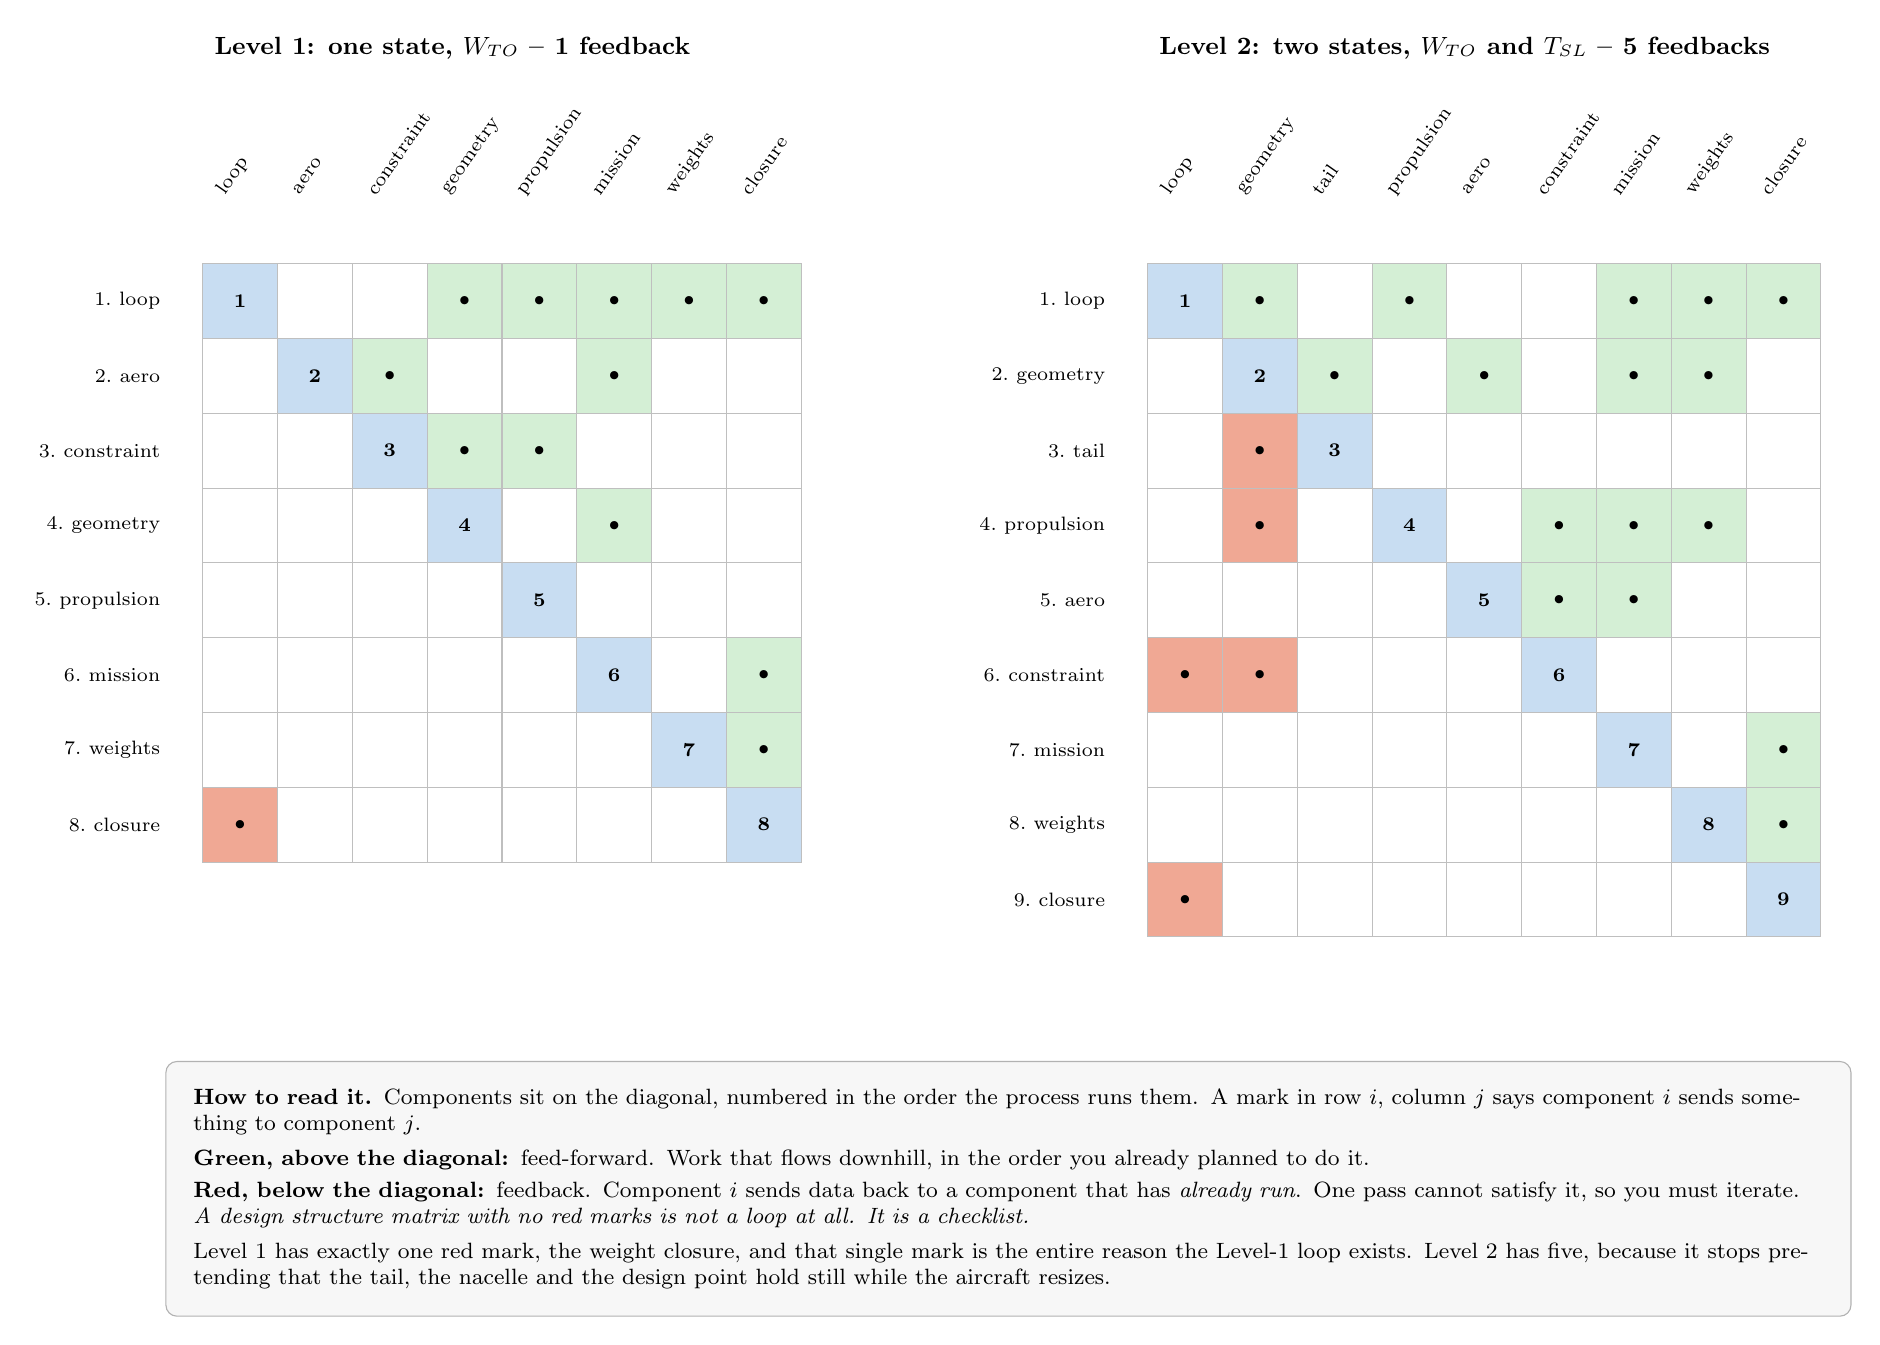
\begin{tikzpicture}

% ======================= LEVEL 1 =========================================
% 1 loop, 2 aero, 3 constraint, 4 geometry, 5 propulsion, 6 mission,
% 7 weights, 8 closure
\begin{scope}[shift={(0,0)}]
  \foreach \i in {1,...,8} \foreach \j in {1,...,8}
      \node[Empty] at (\j*\gs, -\i*\gs) {};
  \foreach \lab [count=\i] in {loop, aero, constraint, geometry, propulsion,
                               mission, weights, closure} {
      \node[RowLab] at (0.3mm, -\i*\gs) {\i.~\lab};
      \node[ColLab] at (\i*\gs - 3mm, 3.5mm) {\lab};
      \node[Comp]   at (\i*\gs, -\i*\gs) {\i};
  }
  % feed-forward, above the diagonal
  \foreach \a/\b in {1/4, 1/5, 1/6, 1/7, 1/8, 2/3, 2/6, 3/4, 3/5, 4/6, 6/8, 7/8}
      \node[Fwd] at (\b*\gs, -\a*\gs) {$\bullet$};
  % feedback, below the diagonal
  \foreach \a/\b in {8/1}
      \node[Back] at (\b*\gs, -\a*\gs) {$\bullet$};
  \node[Ttl] at (5mm, 20mm) {Level 1: one state, $W_{TO}$ -- \textbf{1} feedback};
\end{scope}

% ======================= LEVEL 2 =========================================
% 1 loop, 2 geometry, 3 tail, 4 propulsion, 5 aero, 6 constraint,
% 7 mission, 8 weights, 9 closure
\begin{scope}[shift={(12cm,0)}]
  \foreach \i in {1,...,9} \foreach \j in {1,...,9}
      \node[Empty] at (\j*\gs, -\i*\gs) {};
  \foreach \lab [count=\i] in {loop, geometry, tail, propulsion, aero,
                               constraint, mission, weights, closure} {
      \node[RowLab] at (0.3mm, -\i*\gs) {\i.~\lab};
      \node[ColLab] at (\i*\gs - 3mm, 3.5mm) {\lab};
      \node[Comp]   at (\i*\gs, -\i*\gs) {\i};
  }
  \foreach \a/\b in {1/2, 1/4, 1/7, 1/8, 1/9, 2/3, 2/5, 2/7, 2/8,
                     4/6, 4/7, 4/8, 5/6, 5/7, 7/9, 8/9}
      \node[Fwd] at (\b*\gs, -\a*\gs) {$\bullet$};
  \foreach \a/\b in {3/2, 4/2, 6/1, 6/2, 9/1}
      \node[Back] at (\b*\gs, -\a*\gs) {$\bullet$};
  \node[Ttl] at (5mm, 20mm) {Level 2: two states, $W_{TO}$ and $T_{SL}$ -- \textbf{5} feedbacks};
\end{scope}

% ======================= caption =========================================
\node[align=left, font=\footnotesize, anchor=north west, text width=207mm,
      draw=black!30, fill=black!3, rounded corners, inner sep=3.5mm]
  at (0, -10.6cm)
  {\textbf{How to read it.} Components sit on the diagonal, numbered in the
   order the process runs them. A mark in row~$i$, column~$j$ says component
   $i$ sends something to component~$j$.\\[3pt]
   \textbf{Green, above the diagonal:} feed-forward. Work that flows downhill,
   in the order you already planned to do it.\\[2pt]
   \textbf{Red, below the diagonal:} feedback. Component $i$ sends data back to
   a component that has \emph{already run}. One pass cannot satisfy it, so you
   must iterate. \emph{A design structure matrix with no red marks is not a
   loop at all. It is a checklist.}\\[3pt]
   Level~1 has exactly one red mark, the weight closure, and that single mark
   is the entire reason the Level-1 loop exists. Level~2 has five, because it
   stops pretending that the tail, the nacelle and the design point hold still
   while the aircraft resizes.};

\end{tikzpicture}
\end{document}
